\documentclass[dvisvgm,hypertex,aspectratio=169]{beamer}
\usefonttheme{serif}

%\usepackage[draft]{animate}
\usepackage[final]{animate}
\usepackage{ifthen}


\usepackage{khpreamble}


%%%%%%%%%%%%%%%%%%%%%%%%%%%%%%%%%%%%%%%%%%%%%%%%%%%%%%%%%%%%%%%%%%%%%%%%%%%%%%%
% PageDown, PageUp key event handling; navigation symbols
%%%%%%%%%%%%%%%%%%%%%%%%%%%%%%%%%%%%%%%%%%%%%%%%%%%%%%%%%%%%%%%%%%%%%%%%%%%%%%%
\usepackage[totpages]{zref}
\usepackage{atbegshi}
\usepackage{fontawesome}
\setbeamertemplate{navigation symbols}{}
\AtBeginShipout{%
  \AtBeginShipoutAddToBox{%
    \special{dvisvgm:raw
      <defs>
      <script type="text/javascript">
      <![CDATA[
        document.addEventListener('keydown', function(e){
          if(e.key=='PageDown'){
            \ifnum\thepage<\ztotpages
              document.location.replace('\jobname-\the\numexpr\thepage+1\relax.svg');%
            \fi
          }else if(e.key=='PageUp'){
            \ifnum\thepage>1
            %document.location.replace('\jobname-\the\numexpr\thepage-1\relax.svg');%
              document.location.replace('\jobname-\makeatletter\@anim@pad{2}{\thepage-1}\makeatother\relax.svg');%
            \fi%
          }
        });
      ]]>
      </script>
      </defs>
    }%
  }%
  \AtBeginShipoutUpperLeftForeground{%
    \raisebox{-\dimexpr\height+0.5ex\relax}[0pt][0pt]{\makebox[\paperwidth][r]{%
      \normalsize\color{structure!40!}%
      \ifnum\thepage>1%
      \href{\jobname-\the\numexpr\thepage-1\relax.svg}{\faArrowLeft}%
      \else%  
        \textcolor{lightgray}{\faArrowLeft}%  
      \fi\hspace{0.5ex}%
      \ifnum\thepage<\ztotpages%
      \href{\jobname-\the\numexpr\thepage+1\relax.svg}{\faArrowRight}%
      \else%
        \textcolor{lightgray}{\faArrowRight}%  
      \fi%
      \hspace{0.5ex}%
    }}%
  }%  
}%
%%%%%%%%%%%%%%%%%%%%%%%%%%%%%%%%%%%%%%%%%%%%%%%%%%%%%%%%%%%%%%%%%%%%%%%%%%%%%%%

\usepackage{tikz}
\usepackage{pgfplots}
\usepackage{pgfplotstable}
\pgfplotsset{compat=1.16}
\usetikzlibrary{calc}
\usepackage{amsmath}
\DeclareMathOperator{\sign}{sgn}


\author{Kjartan Halvorsen}
\date{2021-05-19}
\title{Diagrama de bloques}

% ------------------------------------------------
% Determine which slides to include
\includeonlyframes{%
  I0,% Porque algebra de bloques
  MC0,% Modelo compartimentalo
  MC1,% Modelo compartimentalo
  MC2,% Modelo compartimentalo
  H0,% Modelo Hummer
  H1,% Modelo Hummer
}
% ------------------------------------------------

%%%%%%%%%%%%%%%%%%%%%%%%%%%%%%%%%%%%%%%%%%%%%%%%%%%%%%%%%%%%%%%%%%%%%%%%%%%%%%%
% Define footer
\usepackage{ccicons}

\makeatletter
\setbeamertemplate{footline}
{
  \leavevmode%
  \hbox{%
  %\begin{beamercolorbox}[wd=.333333\paperwidth,ht=2.25ex,dp=1ex,center]{title in head/foot}%
    %\usebeamerfont{title in head/foot}\insertsubsection
  %\end{beamercolorbox}%
  %\begin{beamercolorbox}[wd=.333333\paperwidth,ht=2.25ex,dp=1ex,right]{date in head/foot}%
  %  \usebeamerfont{date in head/foot}\insertshortdate{}\hspace*{2em}
  %  \insertframenumber{} / \inserttotalframenumber\hspace*{2ex} 
  %\end{beamercolorbox}}%
  %\vskip0pt%
  \begin{beamercolorbox}[wd=.92\paperwidth,ht=2.25ex,dp=1ex,right]{author in head/foot}%
    \usebeamerfont{author in head/foot}\insertauthor
  \end{beamercolorbox}%
  \begin{beamercolorbox}[wd=.08\paperwidth,ht=2.25ex,dp=1ex,right]{date in head/foot}%
    \ccbysa
  \end{beamercolorbox}}%
  \vskip0pt%
}
\makeatother
%%%%%%%%%%%%%%%%%%%%%%%%%%%%%%%%%%%%%%%%%%%%%%%%%%%%%%%%%%%%%%%%%%%%%%%%%%%%%%%


\newcommand{\hummeranimation}[1]{%

  \def\velocity{1.5}
  \def\startbrake{3}
  \def\braketimeconst{3}

  \begin{center}

  %\begin{animateinline}[controls,autoplay,loop]{20}
  \begin{animateinline}[ ]{28}
      \multiframe{60}{n=0+0.15}{
        \begin{tikzpicture}
          \useasboundingbox (-1 cm, -1 cm) rectangle (9 cm, 3 cm);
          \pgfmathsetmacro{\xpos}{\velocity*\n*(\n<\startbrake) + (\velocity*\startbrake + \velocity*\braketimeconst*(1-(exp(-(\n-\startbrake)/\braketimeconst))))*(\n >= \startbrake)}

            \node[anchor=south,] at (\xpos cm, 0) {\ifnum#1 > 0 \includegraphics[width=15 mm]{hummer-ev.png} \else \tikz \draw[fill, black] (0,0) rectangle (1,1); \fi};
            \draw[->, black!90, semithick] (-1, 0.16) -- (9 , 0.16) node[below, pos=1] {$X$};
        \end{tikzpicture}
      }
    \end{animateinline}
  \end{center}
}

\begin{document}

\maketitle

\begin{frame}[label=I0]{Sistemas de control}

  \begin{center}
    \includegraphics[width=0.7\linewidth]{minchala-block-control.png}\\
    {\tiny Fuente: Prof Ismael Minchala, Tec}
  \end{center}
\end{frame}


\note{%
}

\begin{frame}[label=MC0]{Modelo compartimental}
  \small
  \begin{columns}
    \begin{column}{0.5\linewidth}
      \begin{center}
        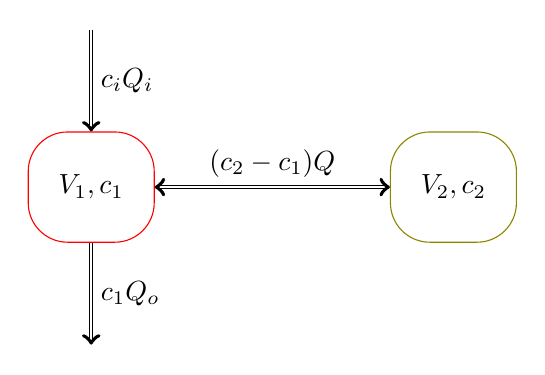
\begin{tikzpicture}[
          compartment/.style={rounded corners=5mm, minimum height=14mm, minimum width=16mm},
          node distance=46mm,
          ]

          \node[compartment, draw=red, ] (comp1) {$V_1, c_1$};
          \node[compartment, right of=comp1, draw=olive,] (comp2) {$V_2, c_2$};

          \node[coordinate, above of=comp1, node distance=20mm] (input) {};
          \node[coordinate, below of=comp1, node distance=20mm] (output) {};

          \draw[->, double] (input) -- node[right]{$c_{i}Q_i$} (comp1);
          \draw[->, double] (comp1) -- node[right]{$c_{1}Q_o$} (output);
          \draw[<->, double] (comp1) -- node[above]{$(c_{2}-c_1)Q$} (comp2);

        \end{tikzpicture}
      \end{center}

    \end{column}
    \begin{column}{0.5\linewidth}
      \begin{equation*}
        \begin{aligned}
          V_1\frac{dc_1}{dt} &= Q(c_2-c_1) - Q_{o}c_1 + Q_ic_{i}, \quad  & c_1 \geq 0 \\
          V_2\frac{dc_2}{dt} &= Q(c_1-c_2),  & c_2 \geq 0,
        \end{aligned}
      \end{equation*}
    \end{column}
  \end{columns}

  \begin{center}
    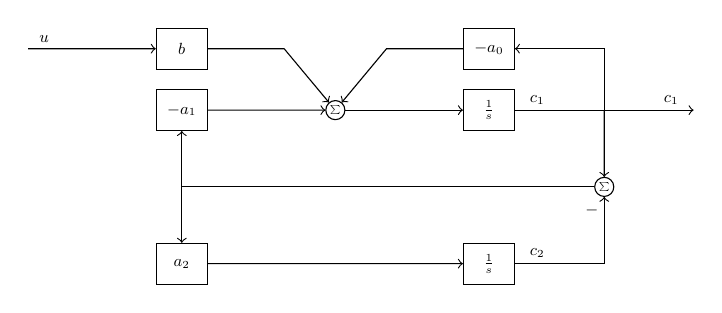
\begin{tikzpicture}[block/.style={rectangle, draw, minimum width=10mm, minimum height=8mm},
      sumnode/.style={circle, draw, inner sep=1pt}, 
      node distance=30mm,
      scale=0.65, transform shape,]
      \small 
      \node[block] (C1int) {$\frac{1}{s}$};
      \node[block, below of=C1int] (C2int) {$\frac{1}{s}$};

      \node[coordinate, right of=C1int, node distance=40mm] (out1) {};
      \draw[->] (C1int) -- node[above, very near start,] {$c_1$} node[coordinate, pos=0.5] (mp) {} node[above, very near end,] {$c_1$} (out1);
      \node[sumnode, below of=mp, node distance=15mm] (sum12) {\tiny $\sum$};
      \draw[->] (mp)  -- node[left, pos=0.9] {} (sum12);
      \draw[->] (C2int)  -| node[above, very near start,] {$c_2$} node[left, pos=0.9] {$-$} (sum12);
      
      \node[sumnode, left of=C1int,] (sum1) {\tiny $\sum$};
      \node[block, above of=C1int, node distance=12mm,] (q0V1) {$-a_0$};

      \node[block, left of=C2int, node distance=60mm] (qV2) {$a_2$};

      \draw[->] (sum12)  -| (qV2);
      \draw[->] (qV2) -- (C2int);

      \node[block, above of=qV2,] (qV1) {$-a_1$};
      \draw[->] (sum12)  -| node[left, pos=0.9] {} (qV1);

      \draw[->] (qV1) -- (sum1);
      \draw[->] (q0V1) -- ++(-20mm, 0) -- (sum1);
      \draw[->] (mp) |- (q0V1);

      \node[block, above of=qV1, node distance=12mm,] (CiV1) {$b$};
      \node[coordinate, left of=CiV1,] (input) {};
      \draw[->] (input) --  node[above, very near start,] {$u$} (CiV1);
      \draw[->] (CiV1) -- ++(20mm, 0) -- (sum1);
      \draw[->] (sum1) -- (C1int);
      

    \end{tikzpicture}
  \end{center}
\end{frame}


\note{%
}

\begin{frame}[label=MC1]{Modelo compartimental}

  \begin{center}
    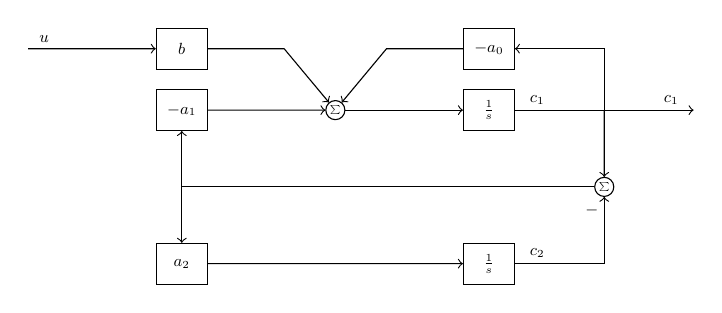
\begin{tikzpicture}[block/.style={rectangle, draw, minimum width=10mm, minimum height=8mm},
      sumnode/.style={circle, draw, inner sep=1pt}, 
      node distance=30mm,
      scale=0.65, transform shape,]
      \small 
      \node[block] (C1int) {$\frac{1}{s}$};
      \node[block, below of=C1int] (C2int) {$\frac{1}{s}$};

      \node[coordinate, right of=C1int, node distance=40mm] (out1) {};
      \draw[->] (C1int) -- node[above, very near start,] {$c_1$} node[coordinate, pos=0.5] (mp) {} node[above, very near end,] {$c_1$} (out1);
      \node[sumnode, below of=mp, node distance=15mm] (sum12) {\tiny $\sum$};
      \draw[->] (mp)  -- node[left, pos=0.9] {} (sum12);
      \draw[->] (C2int)  -| node[above, very near start,] {$c_2$} node[left, pos=0.9] {$-$} (sum12);
      
      \node[sumnode, left of=C1int,] (sum1) {\tiny $\sum$};
      \node[block, above of=C1int, node distance=12mm,] (q0V1) {$-a_0$};

      \node[block, left of=C2int, node distance=60mm] (qV2) {$a_2$};

      \draw[->] (sum12)  -| (qV2);
      \draw[->] (qV2) -- (C2int);

      \node[block, above of=qV2,] (qV1) {$-a_1$};
      \draw[->] (sum12)  -| node[left, pos=0.9] {} (qV1);

      \draw[->] (qV1) -- (sum1);
      \draw[->] (q0V1) -- ++(-20mm, 0) -- (sum1);
      \draw[->] (mp) |- (q0V1);

      \node[block, above of=qV1, node distance=12mm,] (CiV1) {$b$};
      \node[coordinate, left of=CiV1,] (input) {};
      \draw[->] (input) --  node[above, very near start,] {$u$} (CiV1);
      \draw[->] (CiV1) -- ++(20mm, 0) -- (sum1);
      \draw[->] (sum1) -- (C1int);
      

    \end{tikzpicture}
  \end{center}

  \begin{columns}
    \footnotesize
    \begin{column}{0.5\linewidth}
      \begin{align*}
        C_1 &= \frac{1}{s}\big(-a_0C_1 - a_1(C_1-C_2) + bU\Big)\\
        C_2 &= \frac{1}{s}a_2(C_1-C_2)
      \end{align*}
    \end{column}
    \begin{column}{0.5\linewidth}
    \end{column}
  \end{columns}
\end{frame}


\note{%
}

\begin{frame}[label=MC2]{Modelo compartimental}

  \begin{center}
    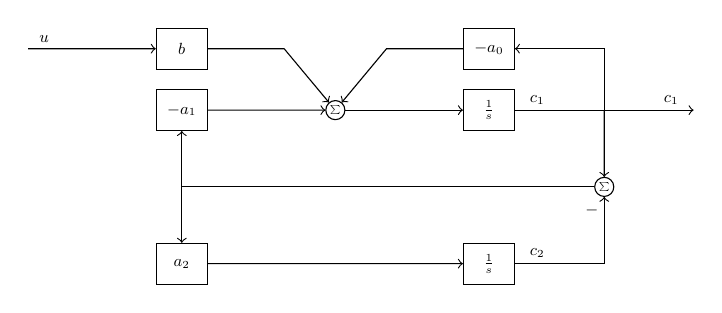
\begin{tikzpicture}[block/.style={rectangle, draw, minimum width=10mm, minimum height=8mm},
      sumnode/.style={circle, draw, inner sep=1pt}, 
      node distance=30mm,
      scale=0.65, transform shape,]
      \small 
      \node[block] (C1int) {$\frac{1}{s}$};
      \node[block, below of=C1int] (C2int) {$\frac{1}{s}$};

      \node[coordinate, right of=C1int, node distance=40mm] (out1) {};
      \draw[->] (C1int) -- node[above, very near start,] {$c_1$} node[coordinate, pos=0.5] (mp) {} node[above, very near end,] {$c_1$} (out1);
      \node[sumnode, below of=mp, node distance=15mm] (sum12) {\tiny $\sum$};
      \draw[->] (mp)  -- node[left, pos=0.9] {} (sum12);
      \draw[->] (C2int)  -| node[above, very near start,] {$c_2$} node[left, pos=0.9] {$-$} (sum12);
      
      \node[sumnode, left of=C1int,] (sum1) {\tiny $\sum$};
      \node[block, above of=C1int, node distance=12mm,] (q0V1) {$-a_0$};

      \node[block, left of=C2int, node distance=60mm] (qV2) {$a_2$};

      \draw[->] (sum12)  -| (qV2);
      \draw[->] (qV2) -- (C2int);

      \node[block, above of=qV2,] (qV1) {$-a_1$};
      \draw[->] (sum12)  -| node[left, pos=0.9] {} (qV1);

      \draw[->] (qV1) -- (sum1);
      \draw[->] (q0V1) -- ++(-20mm, 0) -- (sum1);
      \draw[->] (mp) |- (q0V1);

      \node[block, above of=qV1, node distance=12mm,] (CiV1) {$b$};
      \node[coordinate, left of=CiV1,] (input) {};
      \draw[->] (input) --  node[above, very near start,] {$u$} (CiV1);
      \draw[->] (CiV1) -- ++(20mm, 0) -- (sum1);
      \draw[->] (sum1) -- (C1int);
      

    \end{tikzpicture}
  \end{center}

  \begin{columns}
    \footnotesize
    \begin{column}{0.5\linewidth}
      \begin{align*}
        C_1 &= \frac{1}{s}\big(-a_0C_1 - a_1(C_1-C_2) + bU\Big)\\
        C_2 &= \frac{1}{s}a_2(C_1-C_2)
      \end{align*}
      \begin{align}
        sC_1 + (a_0 + a_1)C_1 &= a_1C_2 + bU  \label{eq:one}\\
        sC_2 + a_2C_2 &= a_2C_1 \label{eq:two}
      \end{align}      

      
      Despejar $C_2$ en \eqref{eq:two} y substituir en \eqref{eq:one}:
    \end{column}
    \begin{column}{0.5\linewidth}
      \begin{align*}
        (s + a_0 + a_1)C_1 &= a_1\frac{a_2C_1}{s+a_2} + bU\\
        (s + a_0 + a_1)(s+a_2)C_1 - a_1a_2C_1 &= b(s+a_2)U\\
        (s^2 + (a_0 + a_1 +a_2)s + a_0a_2 + a_1a_2 - a_1a_2)C_1  &= b(s+a_2)U\\
      \end{align*}
      \[   C_1  = \frac{b(s+a_2)}{s^2 + (a_0 + a_1 +a_2)s  + a_0a_2}U \]

    \end{column}
  \end{columns}
\end{frame}


\note{%
}

  \begin{frame}[label=H0]{Modelo linealizado del Hummer EV}

    \footnotesize

    Parámetros: $m$=5000kg, $C_dA$=2.46, $\rho_a = 1.2$, $C_{rr}$=0.01

  \begin{columns}
    \begin{column}{0.6\linewidth}

      \begin{align*}
        F_d(v) &= r + kv^2 = C_{rr}mg + \frac{1}{2}\rho_a C_d A v^2\\
               &= 0.01\cdot 5000\cdot9.8 + \frac{1}{2}1.2\cdot 2.46 v^2 = 490 + 1.476v^2.
      \end{align*}
      
      \begin{description}
        \pause
      \item[Punto de operación y variables de desviación]
        $v_0 = \unit{22}{\meter\per\second}$, $v=v_0 + y$, $F_m = F_d(v_0) + u$ 
        \pause
      \item[EDO linearizada]
    \[m\dot{y} = -2kv_0y + u,\]
    \[ \frac{5000}{2\cdot 1.476\cdot 22}\dot{y} +  y = \frac{1}{2\cdot 1.476\cdot 22} u, \]
    \[ 77\dot{y} + y = 0.016u. \]
        \pause
  \item[Transformada de Laplace]
    \[ (78.9s + 1) Y(s) = 0.0154 U(s) \]
  \end{description}
\end{column}
\begin{column}{0.4\linewidth}
  \begin{description}
        \pause
  \item[Función de transferencia]
    \[  Y(s) = \underbrace{\frac{\overbrace{0.0154}^K}{ \underbrace{77}_\tau s + 1}}_{G(s)} U(s) \]

        \pause
  \item[Diagrama de bloque]
  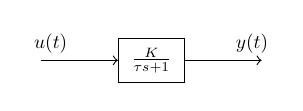
\begin{tikzpicture}[scale=0.7, transform shape, block/.style={draw, minimum width=12mm, minimum height=8mm},]
    \node[block] (plant) {$\frac{K}{\tau s + 1}$};
    \draw[->] (plant) ++ (-2cm, 0) -- node[very near start, above] {$u(t)$} (plant);
    \draw[->] (plant) -- node[very near end, above] {$y(t)$} ++(2cm, 0);
  \end{tikzpicture}
\end{description}
\end{column}
\end{columns}
\end{frame}


\end{document}
